
\section{Modelling of \texorpdfstring{\nb}{Nb} templates with the
  Loose and Light working points}
\label{app:nb_validation_LT}

The likelihood-based validation of the \nb modelling in simulation, as
described in Sec.~\ref{sec:nb-zinv}, is repeated with the \mmj sample
using with Loose and Tight working points, respectively, to check the
validility of the \nb modelling in b-jet-enriched and mistag-enriched
scenarios. The post-fit nuisance parameter values are shown in
Fig.~\ref{fig:loose_tight_nb}. No evidence for mis-modelling is
observed. 

\begin{figure}[h!]
  \centering
  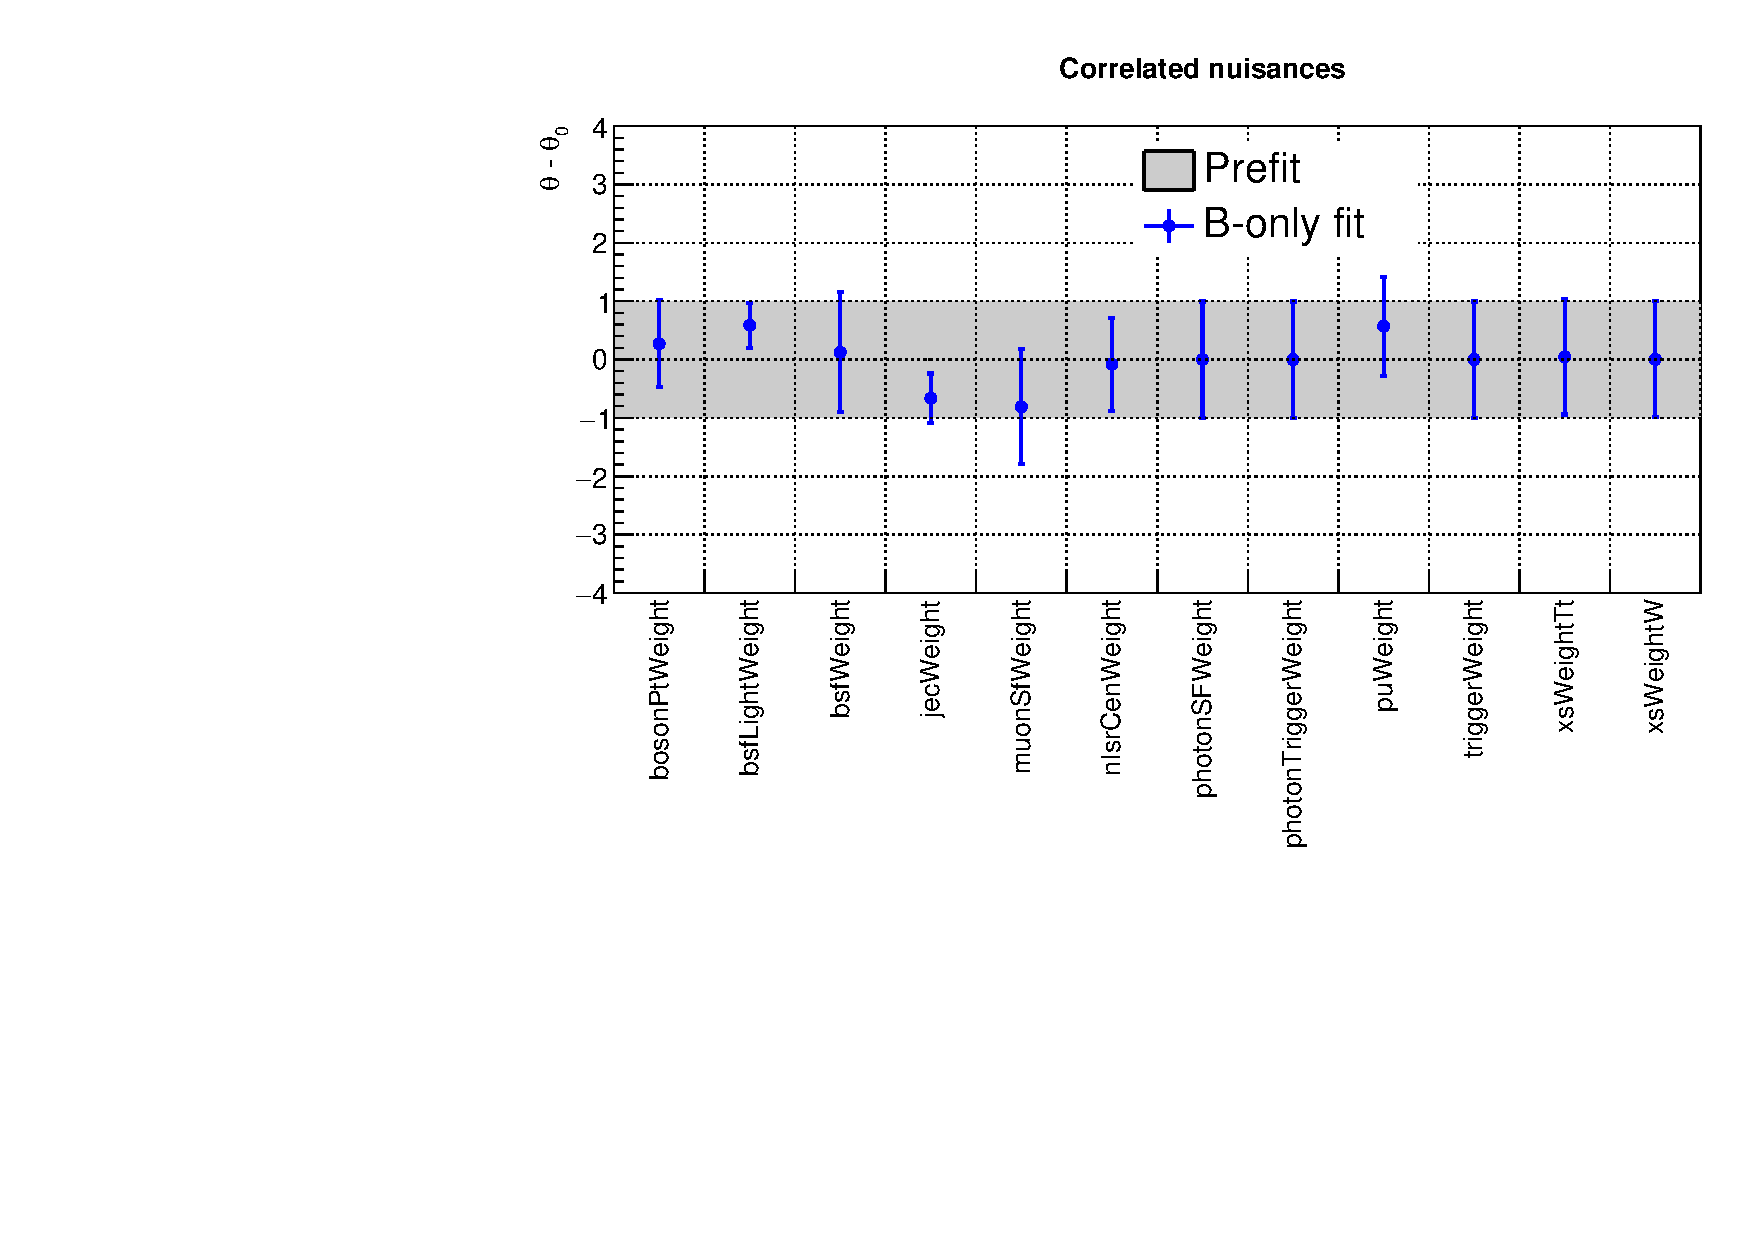
\includegraphics[width=0.6\textwidth]{figures/btag/nuisances/full/Correlated_nuisances_loose}
  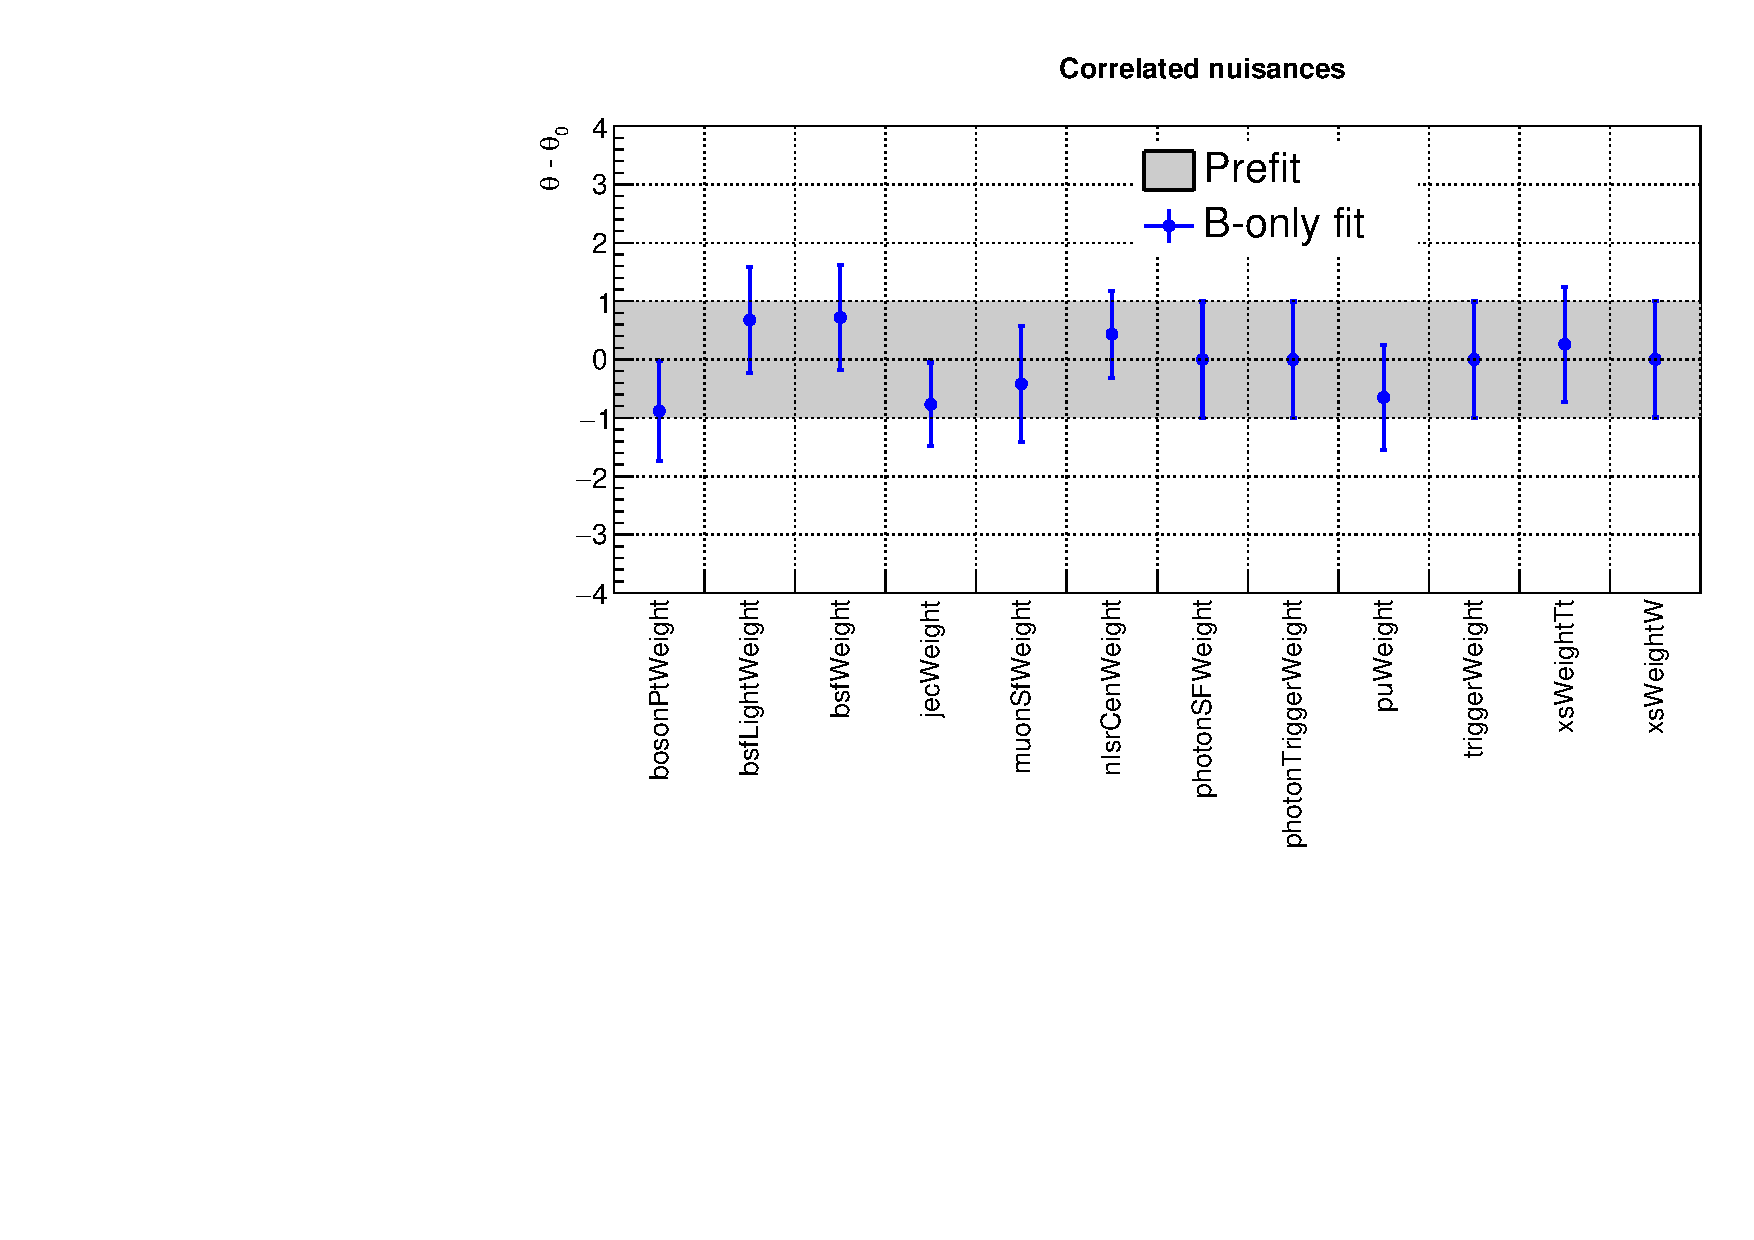
\includegraphics[width=0.6\textwidth]{figures/btag/nuisances/full/Correlated_nuisances_tight}
  \caption{Post-fit nuisances of a likelihood fit to data in the \mmj
    control region with loose (top) and tight (bottom) btagging
    working points. }
  \label{fig:loose_tight_nb}
\end{figure}

